\documentclass[12pt, a4paper]{book}

\usepackage[T1]{fontenc}
\usepackage[utf8]{inputenc}
\usepackage[charter, cal=cmcal]{mathdesign}
\usepackage[scaled=0.92]{helvet}
\usepackage{geometry}
\geometry{a4paper, top=30mm, bottom=30mm, inner=32mm, outer=25mm, marginparwidth=18mm}

\usepackage{amsmath, amsthm}
\usepackage[version=4]{mhchem}
\usepackage{graphicx}
\usepackage[dvipsnames,svgnames,table]{xcolor}
\usepackage{tikz}
\usetikzlibrary{arrows.meta, shapes.geometric, positioning,
                calc, backgrounds, decorations.pathmorphing, patterns}
\usepackage{pgfplots}
\pgfplotsset{compat=1.18}
\usepackage{tcolorbox}
\tcbuselibrary{skins, breakable, theorems}
\usepackage{titlesec}
\usepackage{fancyhdr}
\usepackage{enumitem}
\usepackage{booktabs}
\usepackage{array}
\usepackage{multicol}
\usepackage{caption}
\usepackage{parskip}
\usepackage{siunitx}
\usepackage{pifont}
\usepackage[colorlinks=true, linkcolor=BrickRed,
            urlcolor=NavyBlue, citecolor=ForestGreen]{hyperref}

% ── Colours ───────────────────────────────────────────────────────────────────
\definecolor{JourneyColor}{HTML}{4A235A}
\definecolor{ModuleColor}{HTML}{6C3483}
\definecolor{PuzzleColor}{HTML}{1A5276}
\definecolor{DiscoveryColor}{HTML}{B7950B}
\definecolor{WarningColor}{HTML}{C0392B}
\definecolor{ProblemColor}{HTML}{117A65}
\definecolor{ReflectColor}{HTML}{1D6A39}
\definecolor{HistoryColor}{HTML}{6E2F1A}
\definecolor{LightBg}{HTML}{F8F9FA}
\definecolor{ElectronBlue}{HTML}{1565C0}
\definecolor{NucleusRed}{HTML}{B71C1C}
\definecolor{WaveColor}{HTML}{00695C}

% ── Boxes ─────────────────────────────────────────────────────────────────────
\newtcolorbox{puzzlebox}[1][]{enhanced,breakable,
  colback=PuzzleColor!6,colframe=PuzzleColor,fonttitle=\bfseries\sffamily,
  title={The Puzzle},attach boxed title to top left={yshift=-2mm,xshift=6mm},
  boxed title style={colback=PuzzleColor},borderline west={3pt}{0pt}{PuzzleColor},#1}

\newtcolorbox{discoverybox}[1][]{enhanced,breakable,
  colback=DiscoveryColor!8,colframe=DiscoveryColor,fonttitle=\bfseries\sffamily,
  title={Discovery},attach boxed title to top left={yshift=-2mm,xshift=6mm},
  boxed title style={colback=DiscoveryColor},borderline west={3pt}{0pt}{DiscoveryColor},#1}

\newtcolorbox{problembox}[1][]{enhanced,breakable,
  colback=ProblemColor!5,colframe=ProblemColor,fonttitle=\bfseries\sffamily,
  title={Problems},attach boxed title to top left={yshift=-2mm,xshift=6mm},
  boxed title style={colback=ProblemColor},borderline west={3pt}{0pt}{ProblemColor},#1}

\newtcolorbox{deepbox}[1][]{enhanced,breakable,
  colback=JourneyColor!5,colframe=JourneyColor,fonttitle=\bfseries\sffamily,
  title={Deep Problems},attach boxed title to top left={yshift=-2mm,xshift=6mm},
  boxed title style={colback=JourneyColor},borderline west={4pt}{0pt}{JourneyColor},#1}

\newtcolorbox{historybox}[1][]{enhanced,breakable,
  colback=HistoryColor!7,colframe=HistoryColor!60,fonttitle=\bfseries\sffamily\small,
  title={Historical Note},attach boxed title to top left={yshift=-2mm,xshift=6mm},
  boxed title style={colback=HistoryColor!80},#1}

\newtcolorbox{reflectionbox}[1][]{enhanced,breakable,
  colback=ReflectColor!6,colframe=ReflectColor,fonttitle=\bfseries\sffamily,
  title={Reflection},attach boxed title to top left={yshift=-2mm,xshift=6mm},
  boxed title style={colback=ReflectColor},borderline west={3pt}{0pt}{ReflectColor},#1}

\newtcolorbox{modelbreaks}[1][]{enhanced,breakable,
  colback=WarningColor!6,colframe=WarningColor,fonttitle=\bfseries\sffamily,
  title={Where This Model Breaks},attach boxed title to top left={yshift=-2mm,xshift=6mm},
  boxed title style={colback=WarningColor},borderline west={4pt}{0pt}{WarningColor},#1}

\newtcolorbox{namedconcept}[2][]{enhanced,
  colback=ModuleColor!6,colframe=ModuleColor,fonttitle=\bfseries\sffamily\large,
  title={#2},attach boxed title to top left={yshift=-2mm,xshift=6mm},
  boxed title style={colback=ModuleColor},#1}

% ── Section formatting ────────────────────────────────────────────────────────
\titleformat{\chapter}[display]
  {\normalfont\sffamily\huge\bfseries\color{JourneyColor}}
  {\textcolor{JourneyColor!60}{\chaptertitlename\ \thechapter}}{10pt}{\Huge}
  [\vspace{2pt}\textcolor{JourneyColor}{\titlerule[1.5pt]}]
\titleformat{\section}
  {\normalfont\sffamily\Large\bfseries\color{ModuleColor}}
  {\thesection}{1em}{}[\textcolor{ModuleColor!40}{\titlerule[0.6pt]}]
\titleformat{\subsection}
  {\normalfont\sffamily\large\bfseries\color{JourneyColor!80}}{\thesubsection}{1em}{}
\titleformat{\subsubsection}
  {\normalfont\sffamily\normalsize\bfseries}{\thesubsubsection}{1em}{}

\pagestyle{fancy}
\fancyhf{}
\fancyhead[LE]{\small\sffamily\textcolor{JourneyColor}{\leftmark}}
\fancyhead[RO]{\small\sffamily\textcolor{ModuleColor}{\rightmark}}
\fancyfoot[C]{\small\thepage}
\renewcommand{\headrulewidth}{0.4pt}

\newcommand{\newterm}[1]{\textit{\textcolor{DiscoveryColor}{#1}}}
\newcommand{\important}[1]{\textcolor{ModuleColor}{\textbf{#1}}}

% ══════════════════════════════════════════════════════════════════════════════
\begin{document}
\setcounter{chapter}{1}
\chapter[Journey 2 --- Architecture of the Atom]
        {Journey Two\\[8pt]
         \textcolor{ModuleColor}{\large Architecture of the Atom}}
\setcounter{section}{5}

% ══════════════════════════════════════════════════════════════════════════════
\section{Module 2.6 --- Wave-Particle Duality and the Quantum Atom}
\label{sec:mod2.6}

\subsection*{Motivation}

Bohr's model answered the right questions but for the wrong reasons.
It mixed classical orbits --- electrons following circular paths ---
with quantum postulates --- those orbits do not radiate.
This is logically inconsistent.

The de Broglie picture at the end of Module~2.5 suggested
a resolution: the electron is not a particle in an orbit
but a standing wave around the nucleus.
This module pursues that idea to its logical conclusion.

When we do, we discover something deeper and stranger
than Bohr imagined:
\begin{itemize}[nosep, leftmargin=2em]
  \item Electrons are neither particles nor waves. They are both.
  \item An electron does not have a definite position.
        It has a \emph{probability} of being found at each position.
  \item The act of measuring a position \emph{changes} the state.
  \item The very concept of a trajectory --- position at each moment ---
        does not apply at the quantum scale.
\end{itemize}

This is not philosophy. It is forced on us by experiment.

% ─── Section: de Broglie Matter Waves ────────────────────────────────────────
\subsection{de Broglie's Matter Waves}

In 1924, Louis de Broglie --- a PhD student writing his
doctoral thesis --- proposed that matter has wave properties,
just as light has particle properties.

If a photon with energy $E = hf$ has momentum $p = h/\lambda$,
then by symmetry, any particle with momentum $p$ should have
an associated wavelength:

\begin{namedconcept}{The de Broglie Wavelength (1924)}
\[
  \lambda = \frac{h}{p} = \frac{h}{mv}
\]
Every particle in motion has an associated wavelength.
\begin{itemize}[nosep, leftmargin=2em]
  \item $h = 6.626\times10^{-34}$ J$\cdot$s (Planck's constant)
  \item $p = mv$ (non-relativistic momentum)
  \item For macroscopic objects: $\lambda$ is immeasurably small
  \item For electrons: $\lambda$ is comparable to atomic sizes
\end{itemize}
\end{namedconcept}

\begin{center}
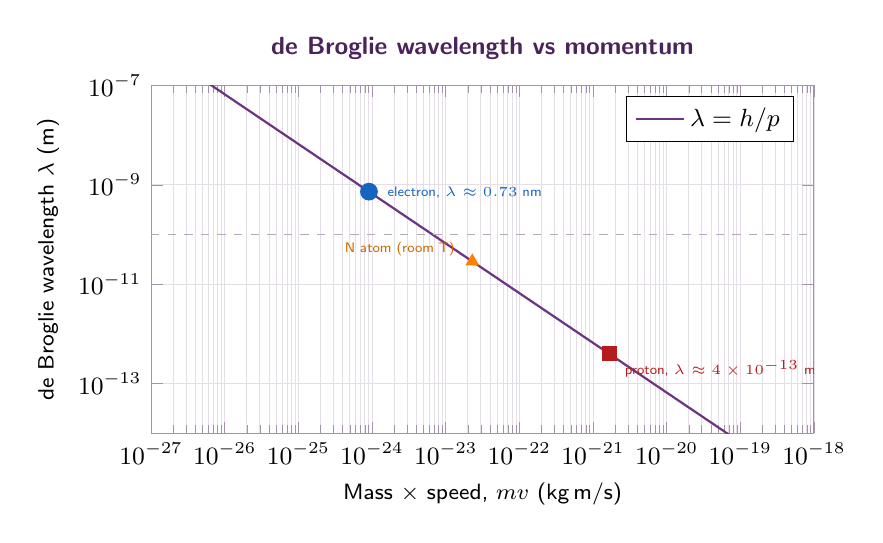
\begin{tikzpicture}[every node/.style={font=\sffamily\small}, scale=1.0]
  \begin{axis}[
    width=10cm, height=6cm,
    xlabel={Mass $\times$ speed, $mv$ (kg\,m/s)},
    ylabel={de Broglie wavelength $\lambda$ (m)},
    xmin=1e-27, xmax=1e-18,
    ymin=1e-14, ymax=1e-7,
    xmode=log, ymode=log,
    grid=both,
    grid style={line width=0.3pt, draw=JourneyColor!15},
    axis line style={color=JourneyColor!50},
    tick style={color=JourneyColor!50},
    title style={font=\sffamily\small\bfseries, color=JourneyColor},
    title={de Broglie wavelength vs momentum},
    label style={font=\sffamily\footnotesize},
    legend style={font=\sffamily\tiny, at={(0.97,0.97)}, anchor=north east}
  ]
    \addplot[thick, color=ModuleColor, domain=1e-27:1e-18, samples=50]
      {6.626e-34/x};
    \addlegendentry{$\lambda = h/p$}

    % Annotate specific particles
    % electron at 1e6 m/s: p = 9.1e-31*1e6 = 9.1e-25
    \addplot[only marks, mark=*, mark size=3pt, color=ElectronBlue]
      coordinates {(9.1e-25, 7.28e-10)};
    \node[font=\sffamily\tiny, text=ElectronBlue, anchor=west]
      at (axis cs:1.2e-24, 7e-10) {electron, $\lambda \approx 0.73$ nm};

    % proton at 1e6 m/s: p = 1.67e-27*1e6 = 1.67e-21
    \addplot[only marks, mark=square*, mark size=2.5pt, color=NucleusRed]
      coordinates {(1.67e-21, 3.97e-13)};
    \node[font=\sffamily\tiny, text=NucleusRed, anchor=west]
      at (axis cs:2e-21, 2e-13) {proton, $\lambda \approx 4\times10^{-13}$ m};

    % atom at thermal speed: nitrogen, ~500 m/s: p = 4.65e-26*500 = 2.3e-23
    \addplot[only marks, mark=triangle*, mark size=2.5pt, color=orange]
      coordinates {(2.3e-23, 2.88e-11)};
    \node[font=\sffamily\tiny, text=orange!80!black, anchor=east]
      at (axis cs:1.8e-23, 5e-11) {N atom (room T)};

    % Atomic size reference
    \draw[dashed, thin, JourneyColor!40]
      (axis cs:1e-27, 1e-10) -- (axis cs:1e-18, 1e-10);
    \node[font=\sffamily\tiny, text=JourneyColor!60, anchor=west]
      at (axis cs:1.2e-18, 1e-10) {atom size};
  \end{axis}
\end{tikzpicture}
\end{center}

\vspace{0.4em}

The electron's de Broglie wavelength in an atom is comparable
to the atom's size.
This is why quantum effects dominate at the atomic scale.
For a baseball (mass 0.14 kg, speed 30 m/s):
$\lambda = h/(mv) \approx 1.6\times10^{-34}$ m ---
a trillion times smaller than a proton.
Quantum effects for baseballs are completely undetectable.

\begin{problembox}
\begin{enumerate}[label=\textbf{\arabic*.}]
  \item Calculate the de Broglie wavelength for:
        \begin{enumerate}[label=(\alph*)]
          \item An electron accelerated through $V = 100$ V.
                (Kinetic energy $= eV$; use $\lambda = h/\sqrt{2m_e eV}$.)
          \item A neutron with kinetic energy 0.025 eV
                (thermal neutron at room temperature).
          \item A $70$ kg person walking at $1.5$ m/s.
          \item A proton in the LHC moving at $0.9999c$
                (use relativistic momentum $p = \gamma m_p v$,
                where $\gamma = 1/\sqrt{1-v^2/c^2}$).
        \end{enumerate}

  \item The electron microscope uses electron waves
        instead of light to image objects.
        \begin{enumerate}[label=(\alph*)]
          \item Light microscopes are limited to resolving
                features larger than $\sim\lambda/2$.
                For green light ($\lambda = 500$ nm),
                what is the resolution limit?
          \item An electron microscope uses electrons
                accelerated through $V = 10$ kV.
                Calculate the electron's de Broglie wavelength.
          \item What is the theoretical resolution of this microscope?
          \item By what factor does the electron microscope
                outresolve a light microscope?
        \end{enumerate}
\end{enumerate}
\end{problembox}

% ─── Section: The Double-Slit Experiment ─────────────────────────────────────
\subsection{The Double-Slit Experiment: The Heart of the Mystery}

The wave nature of matter is most dramatically demonstrated
by the double-slit experiment.

When a beam of electrons is fired at a barrier with
two narrow slits, and the electrons are detected on a screen
beyond, the result is not what classical particle mechanics
predicts.

\begin{center}
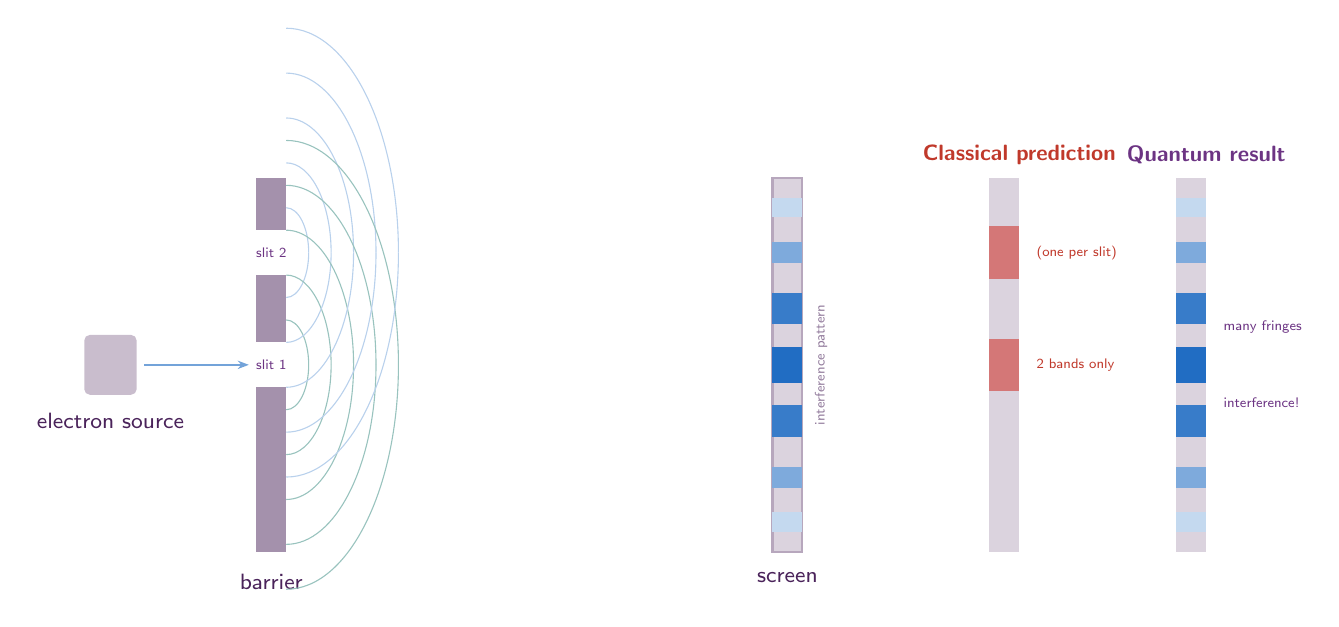
\begin{tikzpicture}[every node/.style={font=\sffamily\small}, scale=0.95]

  % Source
  \fill[JourneyColor!30, rounded corners=2pt]
    (-7.0,-0.4) rectangle (-6.3, 0.4);
  \node[font=\sffamily\footnotesize, text=JourneyColor]
    at (-6.65,-0.75) {electron source};

  % Beam
  \draw[-{Stealth[length=4pt]}, thick, ElectronBlue!60]
    (-6.2,0) -- (-4.8,0);

  % Barrier with two slits
  \fill[JourneyColor!50] (-4.7,-2.5) rectangle (-4.3,-0.3);
  \fill[JourneyColor!50] (-4.7, 0.3) rectangle (-4.3, 1.2);
  \fill[JourneyColor!50] (-4.7, 1.8) rectangle (-4.3, 2.5);
  \node[font=\sffamily\footnotesize, text=JourneyColor]
    at (-4.5,-2.9) {barrier};
  \node[font=\sffamily\tiny, text=ModuleColor]
    at (-4.5,-0.0) {slit 1};
  \node[font=\sffamily\tiny, text=ModuleColor]
    at (-4.5, 1.5) {slit 2};

  % Two sets of expanding wavefronts from each slit
  % Slit 1 at y=0, Slit 2 at y=1.5
  \foreach \r in {0.6, 1.2, 1.8, 2.4, 3.0} {
    \draw[thin, WaveColor!40]
      (-4.3+\r*0.5, 0) arc[start angle=0, end angle=90,
        x radius=\r*0.5, y radius=\r];
    \draw[thin, WaveColor!40]
      (-4.3+\r*0.5, 0) arc[start angle=0, end angle=-90,
        x radius=\r*0.5, y radius=\r];
    \draw[thin, ElectronBlue!30]
      (-4.3+\r*0.5, 1.5) arc[start angle=0, end angle=90,
        x radius=\r*0.5, y radius=\r];
    \draw[thin, ElectronBlue!30]
      (-4.3+\r*0.5, 1.5) arc[start angle=0, end angle=-90,
        x radius=\r*0.5, y radius=\r];
  }

  % Detection screen with interference pattern
  \fill[JourneyColor!20] (2.2,-2.5) rectangle (2.6, 2.5);
  \draw[JourneyColor!40, thick] (2.2,-2.5) rectangle (2.6,2.5);

  % Interference pattern: bright and dark bands
  % Bright at y = 0, +-0.75, +-1.5 (approx)
  % Interference fringes - explicit
  \fill[ElectronBlue!95!white] (2.2,-0.24) rectangle (2.6, 0.24);
  \fill[ElectronBlue!85!white] (2.2, 0.54) rectangle (2.6, 0.96);
  \fill[ElectronBlue!85!white] (2.2,-0.96) rectangle (2.6,-0.54);
  \fill[ElectronBlue!55!white] (2.2, 1.36) rectangle (2.6, 1.64);
  \fill[ElectronBlue!55!white] (2.2,-1.64) rectangle (2.6,-1.36);
  \fill[ElectronBlue!25!white] (2.2, 1.97) rectangle (2.6, 2.23);
  \fill[ElectronBlue!25!white] (2.2,-2.23) rectangle (2.6,-1.97);
  \node[font=\sffamily\footnotesize, text=JourneyColor]
    at (2.4,-2.85) {screen};
  \node[font=\sffamily\tiny, text=JourneyColor!60, rotate=90]
    at (2.85, 0) {interference pattern};

  % What classical particles would give (dots)
  % A separate mini-diagram to the right
  \begin{scope}[xshift=5.5cm]
    \node[font=\sffamily\footnotesize\bfseries, text=WarningColor]
      at (0, 2.8) {Classical prediction};
    \fill[JourneyColor!20] (-0.4,-2.5) rectangle (0,2.5);
    % Only two bands
    \fill[NucleusRed!60] (-0.4,-0.35) rectangle (0,0.35);
    \fill[NucleusRed!60] (-0.4,1.15) rectangle (0,1.85);
    \node[font=\sffamily\tiny, text=WarningColor, anchor=west]
      at (0.1, 0.0) {2 bands only};
    \node[font=\sffamily\tiny, text=WarningColor, anchor=west]
      at (0.1, 1.5) {(one per slit)};
  \end{scope}

  \begin{scope}[xshift=8.0cm]
    \node[font=\sffamily\footnotesize\bfseries, text=ModuleColor]
      at (0, 2.8) {Quantum result};
    \fill[JourneyColor!20] (-0.4,-2.5) rectangle (0,2.5);
    % Quantum fringes explicit
    \fill[ElectronBlue!95!white] (-0.4,-0.24) rectangle (0, 0.24);
    \fill[ElectronBlue!85!white] (-0.4, 0.54) rectangle (0, 0.96);
    \fill[ElectronBlue!85!white] (-0.4,-0.96) rectangle (0,-0.54);
    \fill[ElectronBlue!55!white] (-0.4, 1.36) rectangle (0, 1.64);
    \fill[ElectronBlue!55!white] (-0.4,-1.64) rectangle (0,-1.36);
    \fill[ElectronBlue!25!white] (-0.4, 1.97) rectangle (0, 2.23);
    \fill[ElectronBlue!25!white] (-0.4,-2.23) rectangle (0,-1.97);
    \node[font=\sffamily\tiny, text=ModuleColor, anchor=west]
      at (0.1, 0.5) {many fringes};
    \node[font=\sffamily\tiny, text=ModuleColor, anchor=west]
      at (0.1,-0.5) {interference!};
  \end{scope}

\end{tikzpicture}
\end{center}

\vspace{0.5em}

The experiment has been done with electrons, atoms, even large
molecules ($C_{60}$ buckminsterfullerene, mass $\sim 720$ u).
The interference pattern always appears.

\begin{puzzlebox}
The double-slit experiment has a deeply disturbing feature.

\begin{enumerate}[label=(\alph*), leftmargin=*]
  \item If you fire electrons one at a time --- so slowly that
        only one electron is in the apparatus at any moment ---
        does the interference pattern still appear?
        Write your prediction before reading on.

  \item It does. Each individual electron somehow ``interferes
        with itself.'' After thousands of electrons, each
        landing at a seemingly random position, the
        \emph{statistical pattern} of where they land builds
        up into the interference fringes.

        What does this tell us about the path the electron
        takes through the apparatus?
        Can we say it went through slit 1, or slit 2?

  \item Now suppose we place a detector at the slits to find
        out which slit each electron passes through.
        We watch carefully: electron A went through slit 1.
        Electron B went through slit 2.

        The interference pattern \emph{disappears}.
        It is replaced by two classical bands.

        What does this tell us about the relationship between
        measurement and quantum state?

  \item Richard Feynman said the double-slit experiment contains
        ``the only mystery'' of quantum mechanics.
        What is the mystery? Write it in one sentence,
        as precisely as you can.
\end{enumerate}
\end{puzzlebox}

% ─── Section: The Wave Function ───────────────────────────────────────────────
\subsection{The Wave Function: Probability in Space}

Quantum mechanics describes a particle not by a position
and velocity, but by a \newterm{wave function} $\psi(\mathbf{r}, t)$.

The wave function is a complex-valued function of position
and time.
Its physical meaning, given by Max Born (1926), is:

\begin{namedconcept}{The Born Interpretation of the Wave Function}
The probability of finding the particle at position
$\mathbf{r}$ at time $t$ is proportional to
$|\psi(\mathbf{r},t)|^2$.

More precisely, the probability of finding the particle
in a small volume $dV$ around position $\mathbf{r}$ is:
\[
  dP = |\psi(\mathbf{r},t)|^2\, dV
\]

The wave function must be \newterm{normalised}:
\[
  \int_{\text{all space}} |\psi|^2\, dV = 1
\]
(total probability of finding the particle somewhere $= 1$).
\end{namedconcept}

\vspace{0.5em}

The quantity $|\psi|^2$ is called the
\newterm{probability density}.
It tells us where the electron is \emph{likely} to be found,
not where it \emph{is}.

Before measurement, the electron does not have a definite
position --- it exists in a superposition of all positions
weighted by the probability density.
After measurement, the wave function \newterm{collapses}
to a sharp position.

This is not a limitation of our instruments.
It is a fundamental feature of nature.

% ─── Section: Heisenberg Uncertainty ─────────────────────────────────────────
\subsection{The Heisenberg Uncertainty Principle}

In 1927, Werner Heisenberg derived a fundamental limit
on how precisely position and momentum can both be known
simultaneously:

\begin{namedconcept}{Heisenberg Uncertainty Principle}
\[
  \Delta x \cdot \Delta p_x \geq \frac{\hbar}{2}
\]
where $\Delta x$ is the uncertainty in position,
$\Delta p_x$ is the uncertainty in momentum in the same direction,
and $\hbar = h/2\pi$.

A second relation connects energy and time:
\[
  \Delta E \cdot \Delta t \geq \frac{\hbar}{2}
\]

These are not limitations of measurement technology.
They are fundamental properties of wave-like systems.
\end{namedconcept}

\vspace{0.5em}

The uncertainty principle is a consequence of the wave
nature of matter.
A wave with a precise wavelength (precise momentum)
extends over all space (completely uncertain position).
A wave localised to a small region (precise position)
is built from a superposition of many wavelengths
(uncertain momentum).

\begin{center}
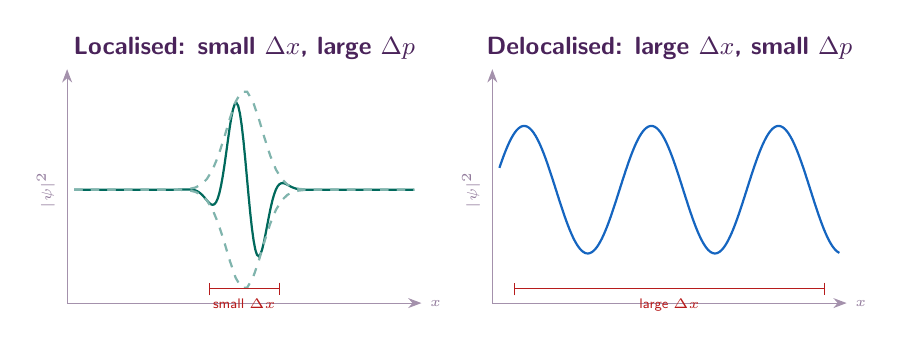
\begin{tikzpicture}[every node/.style={font=\sffamily\small}, scale=0.9]

  % Left: narrow wave packet - precise position, uncertain momentum
  \begin{scope}[xshift=-5.5cm]
    \node[font=\sffamily\small\bfseries, text=JourneyColor]
      at (2.5, 2.0) {Localised: small $\Delta x$, large $\Delta p$};
    \draw[-{Stealth}, thin, JourneyColor!50] (0,-1.6) -- (5.0,-1.6);
    \draw[-{Stealth}, thin, JourneyColor!50] (0,-1.6) -- (0, 1.7);
    \node[font=\sffamily\tiny, text=JourneyColor!60] at (5.2,-1.6) {$x$};
    \node[font=\sffamily\tiny, text=JourneyColor!60, rotate=90]
      at (-0.3, 0) {$|\psi|^2$};
    % Gaussian-like packet
    \draw[thick, WaveColor, domain=0.1:4.9, samples=200]
      plot(\x, {1.4*exp(-8*(\x-2.5)^2)*cos(8*\x r)+0.0});
    \draw[thick, WaveColor!50, dashed, domain=0.1:4.9, samples=60]
      plot(\x, {1.4*exp(-8*(\x-2.5)^2)});
    \draw[thick, WaveColor!50, dashed, domain=0.1:4.9, samples=60]
      plot(\x, {-1.4*exp(-8*(\x-2.5)^2)});
    % Delta x annotation
    \draw[{|}-{|}, thin, NucleusRed] (2.0,-1.4) -- (3.0,-1.4)
      node[midway, below, font=\sffamily\tiny, text=NucleusRed]
        {small $\Delta x$};
  \end{scope}

  % Right: extended wave - uncertain position, precise momentum
  \begin{scope}[xshift=0.5cm]
    \node[font=\sffamily\small\bfseries, text=JourneyColor]
      at (2.5, 2.0) {Delocalised: large $\Delta x$, small $\Delta p$};
    \draw[-{Stealth}, thin, JourneyColor!50] (0,-1.6) -- (5.0,-1.6);
    \draw[-{Stealth}, thin, JourneyColor!50] (0,-1.6) -- (0, 1.7);
    \node[font=\sffamily\tiny, text=JourneyColor!60] at (5.2,-1.6) {$x$};
    \node[font=\sffamily\tiny, text=JourneyColor!60, rotate=90]
      at (-0.3, 0) {$|\psi|^2$};
    % Single-frequency wave
    \draw[thick, ElectronBlue, domain=0.1:4.9, samples=200]
      plot(\x, {0.9*sin(3.5*\x r)});
    % Delta x annotation
    \draw[{|}-{|}, thin, NucleusRed] (0.3,-1.4) -- (4.7,-1.4)
      node[midway, below, font=\sffamily\tiny, text=NucleusRed]
        {large $\Delta x$};
  \end{scope}

\end{tikzpicture}
\end{center}

\vspace{0.5em}

The uncertainty principle explains why atoms don't collapse
without invoking Bohr's ad-hoc postulate.

\begin{discoverybox}
\textbf{Why atoms don't collapse: the uncertainty principle argument.}

If the electron fell to the nucleus (radius $\sim 10^{-15}$ m),
its position would be known to within $\Delta x \sim 10^{-15}$ m.
By the uncertainty principle:
\[
  \Delta p \geq \frac{\hbar}{2\Delta x}
        = \frac{1.055\times10^{-34}}{2\times10^{-15}}
        \approx 5\times10^{-20}\ \text{kg\,m/s}
\]
The minimum kinetic energy from this momentum uncertainty is:
\[
  K \geq \frac{(\Delta p)^2}{2m_e}
        \approx \frac{(5\times10^{-20})^2}{2\times9.1\times10^{-31}}
        \approx 1.4\times10^{-9}\ \text{J} \approx 8700\ \text{eV}
\]
The electrostatic binding energy at the nuclear surface is only
about $-14$ keV for hydrogen.
At the actual ground state radius ($\sim 5\times10^{-11}$ m),
the balance of kinetic energy (from uncertainty) and potential energy
reaches a minimum --- the stable ground state.

The electron doesn't fall into the nucleus because
\emph{localising it more would cost more kinetic energy than
the potential energy gained}.
\end{discoverybox}

\begin{problembox}
\begin{enumerate}[label=\textbf{\arabic*.}]
  \item Use the uncertainty principle to estimate the
        ground-state energy of hydrogen.
        \begin{enumerate}[label=(\alph*)]
          \item If the electron is confined to a region
                of size $\sim r$ (the orbital radius),
                use $\Delta x \sim r$ to estimate $\Delta p$.
          \item The minimum kinetic energy is
                $K \approx (\Delta p)^2/(2m_e)$.
                Express $K$ in terms of $r$.
          \item The potential energy is
                $V = -e^2/(4\pi\varepsilon_0 r)$.
                Write the total energy $E = K + V$.
          \item Minimise $E$ with respect to $r$ to find
                the most stable radius.
                What value do you get?
                Compare to the Bohr radius $a_0 = 0.529$ \AA.
          \item What is the minimum energy? Compare to $-13.6$ eV.
        \end{enumerate}

  \item An electron is confined in a box of width
        $L = 1.0\times10^{-10}$ m (roughly atomic size).
        \begin{enumerate}[label=(\alph*)]
          \item Estimate $\Delta p$ using $\Delta x \approx L$.
          \item Estimate the minimum kinetic energy in eV.
          \item What does this tell you about the typical
                kinetic energies of electrons in atoms?
        \end{enumerate}

  \item The energy-time uncertainty applies to excited states.
        An excited atom emits a photon and drops to ground state.
        If the excited-state lifetime is $\tau = 10^{-9}$ s:
        \begin{enumerate}[label=(\alph*)]
          \item Estimate $\Delta E$ for the excited state.
          \item If the photon has energy $E_0 = 2.1$ eV
                (corresponding to a sharp frequency),
                estimate the fractional spread in frequency
                $\Delta\nu/\nu$.
          \item This spread is called \newterm{natural linewidth}.
                Why do spectral lines have finite width,
                and what sets the minimum width?
        \end{enumerate}
\end{enumerate}
\end{problembox}

% ─── Section: The Schrödinger Equation ───────────────────────────────────────
\subsection{The Schr\"{o}dinger Equation: The Law Governing Waves}

In 1926, Erwin Schr\"{o}dinger wrote down the equation
that governs how quantum wave functions evolve.
It plays the same role in quantum mechanics that Newton's
second law plays in classical mechanics --- it tells you
how the state of a system changes.

For a single particle in a potential $V(\mathbf{r})$,
the time-independent Schr\"{o}dinger equation is:

\begin{namedconcept}{The Schr\"{o}dinger Equation (1926)}
\[
  -\frac{\hbar^2}{2m}\nabla^2\psi + V\psi = E\psi
\]
Or in one dimension:
\[
  -\frac{\hbar^2}{2m}\frac{d^2\psi}{dx^2} + V(x)\psi(x) = E\psi(x)
\]
\begin{itemize}[nosep, leftmargin=2em]
  \item $\psi(x)$ --- the wave function (determines probabilities)
  \item $V(x)$ --- the potential energy (e.g.\ Coulomb for hydrogen)
  \item $E$ --- the total energy (an eigenvalue)
  \item $m$ --- the particle mass
  \item $\hbar = h/2\pi$ --- reduced Planck constant
\end{itemize}
\end{namedconcept}

\vspace{0.5em}

We will not solve this equation in full generality here
(that is the subject of Module~2.7).
But we can understand its key message.

The equation says: \emph{only certain values of $E$ allow
a physically reasonable (normalisable) wave function to exist.}

These allowed energies are the quantum energy levels.
Quantisation is not postulated, as in Bohr's model ---
it \emph{emerges automatically} from requiring the wave
function to be well-behaved.

\subsubsection{Particle in a Box: The Simplest Case}

Consider a particle confined to a one-dimensional box
of length $L$ with perfectly rigid walls.
The potential is:
\[
  V(x) = 0 \quad (0 < x < L), \qquad V = \infty \quad \text{outside}
\]

Inside the box, $\psi$ must be zero at the walls
(the wave cannot penetrate infinite walls).
The solutions are standing waves:

\[
  \psi_n(x) = \sqrt{\frac{2}{L}}\sin\!\left(\frac{n\pi x}{L}\right)
  \qquad n = 1, 2, 3, \ldots
\]

with energies:
\[
  E_n = \frac{n^2 \pi^2 \hbar^2}{2mL^2} = \frac{n^2 h^2}{8mL^2}
\]

\begin{center}
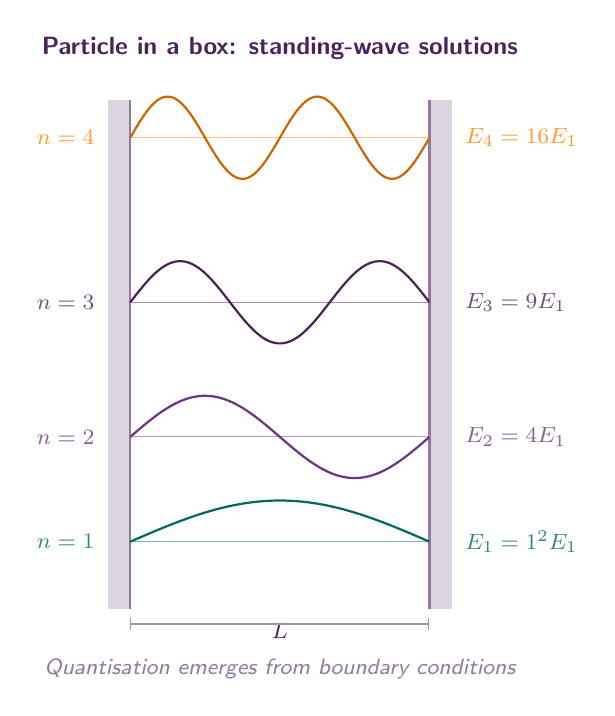
\begin{tikzpicture}[every node/.style={font=\sffamily\small}, scale=0.95]

  % Box walls
  \fill[JourneyColor!20] (-0.3,-0.3) rectangle (0,6.5);
  \fill[JourneyColor!20] (4.0,-0.3) rectangle (4.3,6.5);
  \draw[thick, JourneyColor!60] (0,-0.3) -- (0,6.5);
  \draw[thick, JourneyColor!60] (4.0,-0.3) -- (4.0,6.5);
  \node[font=\sffamily\footnotesize, text=JourneyColor]
    at (2.0,-0.6) {$L$};
  \draw[{|}-{|}, thin, JourneyColor!50] (0,-0.5) -- (4.0,-0.5);

  % Energy levels and wave functions
  % n=1: E1, at height y=0.5; n=2: y=2.0; n=3: y=4.0; n=4: y=6.0
  \pgfmathsetmacro{\Eo}{0.8}  % E1 in plot units
  % n=1
  \draw[thin, WaveColor!50] (0,0.6) -- (4.0,0.6);
  \node[left, font=\sffamily\footnotesize, text=WaveColor!80] at (-0.35,0.6) {$n=1$};
  \node[right, font=\sffamily\footnotesize, text=WaveColor!80] at (4.35,0.6) {$E_1=1^2 E_1$};
  \draw[thick, WaveColor, domain=0:4.0, samples=100]
    plot(\x, {0.6 + 0.55*sin(1*pi*\x/4 r)});
  % n=2
  \draw[thin, ModuleColor!50] (0,2.0) -- (4.0,2.0);
  \node[left, font=\sffamily\footnotesize, text=ModuleColor!80] at (-0.35,2.0) {$n=2$};
  \node[right, font=\sffamily\footnotesize, text=ModuleColor!80] at (4.35,2.0) {$E_2=4E_1$};
  \draw[thick, ModuleColor, domain=0:4.0, samples=100]
    plot(\x, {2.0 + 0.55*sin(2*pi*\x/4 r)});
  % n=3
  \draw[thin, JourneyColor!50] (0,3.8) -- (4.0,3.8);
  \node[left, font=\sffamily\footnotesize, text=JourneyColor!80] at (-0.35,3.8) {$n=3$};
  \node[right, font=\sffamily\footnotesize, text=JourneyColor!80] at (4.35,3.8) {$E_3=9E_1$};
  \draw[thick, JourneyColor, domain=0:4.0, samples=100]
    plot(\x, {3.8 + 0.55*sin(3*pi*\x/4 r)});
  % n=4
  \draw[thin, orange!50] (0,6.0) -- (4.0,6.0);
  \node[left, font=\sffamily\footnotesize, text=orange!80] at (-0.35,6.0) {$n=4$};
  \node[right, font=\sffamily\footnotesize, text=orange!80] at (4.35,6.0) {$E_4=16E_1$};
  \draw[thick, orange!80!black, domain=0:4.0, samples=100]
    plot(\x, {6.0 + 0.55*sin(4*pi*\x/4 r)});

  % Label
  \node[font=\sffamily\small\bfseries, color=JourneyColor]
    at (2.0, 7.2) {Particle in a box: standing-wave solutions};
  \node[font=\sffamily\footnotesize\itshape, text=JourneyColor!60]
    at (2.0, -1.1) {Quantisation emerges from boundary conditions};

\end{tikzpicture}
\end{center}

\vspace{0.5em}

The key point: the boundary condition (wave must be zero
at the walls) forces $n$ to be a positive integer.
The energy is quantised --- not assumed, but \emph{derived}.

For the hydrogen atom, the same logic applies with the
Coulomb potential instead of the box walls.
The boundary condition is that $\psi \to 0$ as $r \to \infty$
(the electron is bound).
This forces the energy to take only the values
$E_n = -13.6/n^2$ eV --- exactly Bohr's result,
without Bohr's ad-hoc postulates.

\begin{historybox}
\textbf{Schr\"{o}dinger vs Heisenberg: Two Routes to Quantum Mechanics}

Quantum mechanics was discovered twice, simultaneously,
in completely different mathematical form.

In 1925, Werner Heisenberg invented \emph{matrix mechanics}:
physical quantities (position, momentum) are represented
as matrices, and time evolution is given by matrix equations.
It was algebraically powerful but physically opaque.

In 1926, Erwin Schr\"{o}dinger invented \emph{wave mechanics}:
the wave function evolves according to a differential equation.
It was physically intuitive but mathematically different.

Both gave the same answers for every observable quantity.
Schr\"{o}dinger and Heisenberg disliked each other intensely.

Paul Dirac and others quickly showed the two approaches were
mathematically equivalent --- just different representations
of the same abstract theory.
The unified formulation became quantum mechanics as we know it.

Heisenberg received the Nobel Prize in 1932.
Schr\"{o}dinger shared it with Paul Dirac in 1933.
\end{historybox}

% ─── Section: The Hydrogen Wave Functions ────────────────────────────────────
\subsection{Hydrogen Wave Functions: Probability Clouds}

When the Schr\"{o}dinger equation is solved for the
hydrogen atom (Coulomb potential), the wave functions
depend on three quantum numbers: $n$, $\ell$, $m_\ell$.

The probability density $|\psi|^2$ describes where
the electron is likely to be found.
These are often visualised as \newterm{probability clouds}
or \newterm{electron density plots}.

\begin{center}
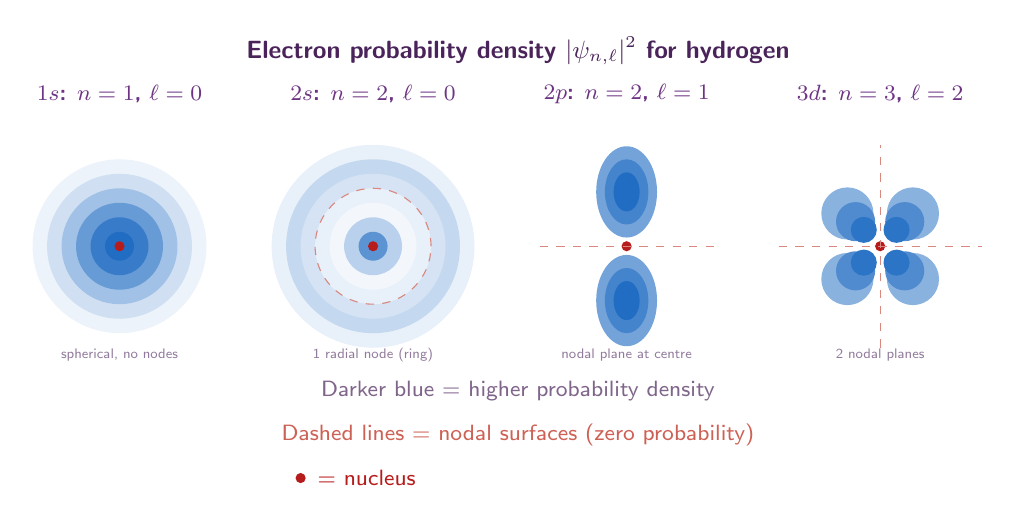
\begin{tikzpicture}[every node/.style={font=\sffamily\small}, scale=0.92]

  \node[font=\sffamily\small\bfseries, color=JourneyColor]
    at (6.5, 6.5) {Electron probability density $|\psi_{n,\ell}|^2$
                   for hydrogen};

  % 1s orbital
  \begin{scope}[xshift=1.0cm, yshift=3.8cm]
    \node[font=\sffamily\footnotesize\bfseries, color=ModuleColor]
      at (0, 2.1) {$1s$: $n=1$, $\ell=0$};
    % Circular gradient
    \foreach \r/\op in {
      1.2/8, 1.0/20, 0.8/40, 0.6/65, 0.4/85, 0.2/95
    }{
      \fill[ElectronBlue!\op] (0,0) circle (\r cm);
    }
    \fill[NucleusRed] (0,0) circle (0.07cm);
    \node[font=\sffamily\tiny, text=JourneyColor!60]
      at (0,-1.5) {spherical, no nodes};
  \end{scope}

  % 2s orbital
  \begin{scope}[xshift=4.5cm, yshift=3.8cm]
    \node[font=\sffamily\footnotesize\bfseries, color=ModuleColor]
      at (0, 2.1) {$2s$: $n=2$, $\ell=0$};
    \foreach \r/\op in {
      1.4/10, 1.2/25, 1.0/18, 0.8/10, 0.6/5, 0.4/30, 0.2/70
    }{
      \fill[ElectronBlue!\op] (0,0) circle (\r cm);
    }
    % Nodal sphere ring
    \draw[thin, WarningColor!60, dashed] (0,0) circle (0.8cm);
    \fill[NucleusRed] (0,0) circle (0.07cm);
    \node[font=\sffamily\tiny, text=JourneyColor!60]
      at (0,-1.5) {1 radial node (ring)};
  \end{scope}

  % 2p orbital
  \begin{scope}[xshift=8.0cm, yshift=3.8cm]
    \node[font=\sffamily\footnotesize\bfseries, color=ModuleColor]
      at (0, 2.1) {$2p$: $n=2$, $\ell=1$};
    % Two lobes along z-axis
    \foreach \sc/\ycen in {0.9/0.75, 0.9/-0.75}{
      \foreach \r/\op in {0.7/60, 0.5/80, 0.3/95}{
        \fill[ElectronBlue!\op] (0,\ycen) ellipse ({\r*0.6} and {\r*\sc});
      }
    }
    \fill[NucleusRed] (0,0) circle (0.07cm);
    \draw[thin, WarningColor!60, dashed] (-1.2,0) -- (1.2,0);
    \node[font=\sffamily\tiny, text=JourneyColor!60]
      at (0,-1.5) {nodal plane at centre};
  \end{scope}

  % 3d orbital
  \begin{scope}[xshift=11.5cm, yshift=3.8cm]
    \node[font=\sffamily\footnotesize\bfseries, color=ModuleColor]
      at (0, 2.1) {$3d$: $n=3$, $\ell=2$};
    % Four lobes (cloverleaf pattern, 2D approximation)
    \foreach \angle in {45, 135, 225, 315}{
      \foreach \r/\op in {0.8/50, 0.6/75, 0.4/90}{
        \fill[ElectronBlue!\op]
          ({\r*0.8*cos(\angle)},{\r*0.8*sin(\angle)})
          ellipse ({\r*0.45} and {\r*0.45});
      }
    }
    \fill[NucleusRed] (0,0) circle (0.07cm);
    \draw[thin, WarningColor!60, dashed] (-1.4,0) -- (1.4,0);
    \draw[thin, WarningColor!60, dashed] (0,-1.4) -- (0,1.4);
    \node[font=\sffamily\tiny, text=JourneyColor!60]
      at (0,-1.5) {2 nodal planes};
  \end{scope}

  % Legend
  \node[font=\sffamily\footnotesize, text=JourneyColor!70]
    at (6.5, 1.8) {Darker blue = higher probability density};
  \node[font=\sffamily\footnotesize, text=WarningColor!80]
    at (6.5, 1.2) {Dashed lines = nodal surfaces (zero probability)};
  \fill[NucleusRed] (3.5, 0.6) circle (0.07cm);
  \node[font=\sffamily\footnotesize, text=NucleusRed, right]
    at (3.6, 0.6) {= nucleus};

\end{tikzpicture}
\end{center}

\vspace{0.5em}

This is the modern picture of the atom.
There are no orbits.
There are only probability distributions.
The electron in a hydrogen 1$s$ state is most likely
to be found at $r = a_0$ from the nucleus,
but it can be found anywhere from $r = 0$ to $r = \infty$,
with probability decreasing away from the peak.

% ─── Section: Deep Problems ───────────────────────────────────────────────────
\subsection*{Deep Problems}

\begin{deepbox}
\begin{enumerate}[label=\textbf{D\arabic*.}]

  \item \textbf{Electron Diffraction.}

        Davisson and Germer (1927) confirmed de Broglie's
        hypothesis by reflecting electrons off a crystal
        of nickel.
        The crystal lattice acts as a diffraction grating
        with spacing $d = 2.15\times10^{-10}$ m.
        Electrons accelerated through $V = 54$ V were
        reflected, and a strong peak appeared at angle
        $\theta = 50°$ from the surface.

        The Bragg diffraction condition is:
        $2d\sin\theta = n\lambda$ (for constructive interference).

        \begin{enumerate}[label=(\alph*)]
          \item Calculate the kinetic energy and momentum of
                the electrons.
          \item Calculate the de Broglie wavelength.
          \item Using the Bragg condition with $n=1$,
                calculate the angle at which a maximum should
                appear.
                Compare to the observed $50°$.
          \item This was the first direct experimental proof
                of matter waves.
                Explain why this experiment is more direct
                evidence than Bohr's model.
        \end{enumerate}

  \item \textbf{Uncertainty and Nuclear Confinement.}

        Nucleons (protons and neutrons) are confined within
        the nucleus to a region of radius
        $r_\text{nuc} \approx 1.5\times10^{-15}$ m.

        \begin{enumerate}[label=(\alph*)]
          \item Estimate the minimum momentum of a nucleon
                confined to this region.
          \item Estimate the minimum kinetic energy in MeV.
                (Use $K = p^2/(2m_p)$,
                $m_p = 1.67\times10^{-27}$ kg.)
          \item This energy is enormous compared to the
                binding energy per nucleon ($\sim 8$ MeV).
                What does this tell us about nuclear binding?
          \item Now apply the same calculation to an electron
                confined to the nucleus.
                Calculate the minimum electron kinetic energy.
          \item Before the neutron was discovered, some physicists
                thought nuclei might contain electrons.
                Use your answer from (d) to explain why
                this is impossible.
        \end{enumerate}

  \item \textbf{The Particle in a Box as a Model Atom.}

        Treat an electron confined to a one-dimensional box
        of width $L$ as a rough model for an atom.

        \begin{enumerate}[label=(\alph*)]
          \item The energy levels are $E_n = n^2 h^2/(8m_eL^2)$.
                For what box size $L$ does the $n=1$ energy
                equal the hydrogen ground state energy ($-13.6$ eV)?
                Compare to $a_0$.
          \item The first excitation energy ($n=1 \to n=2$)
                of the box is $3E_1$.
                Calculate this for the $L$ found in (a)
                and compare to the $n=1\to n=2$ gap in hydrogen
                (10.2 eV).
          \item \emph{Conjugated molecules} like beta-carotene
                (a pigment responsible for orange colour)
                have delocalised $\pi$-electrons that can
                be modelled as a particle in a box.
                Beta-carotene has 11 conjugated double bonds,
                with effective box length $L \approx 1.8$ nm.
                There are 22 $\pi$-electrons, filling levels
                up to $n=11$ (2 per level).
                The lowest-energy transition is $n=11\to n=12$.
                Calculate the wavelength of this transition.
                In what colour region does it fall?
                (Beta-carotene absorbs blue-violet and transmits
                orange --- does this match?)
        \end{enumerate}

\end{enumerate}
\end{deepbox}

% ─── Reflection ───────────────────────────────────────────────────────────────
\subsection*{Reflection}

\begin{reflectionbox}
\begin{enumerate}[label=\textbf{R\arabic*.}]
  \item The Copenhagen interpretation of quantum mechanics says
        the wave function does not describe what the electron
        \emph{is}, only what we will \emph{observe} when we measure it.
        The electron has no definite position before measurement.
        \textbf{Does this mean the electron doesn't exist before
        measurement?} What does ``existence'' mean for a quantum
        particle? Is this a scientific question or a philosophical one?

  \item Classical physics is \emph{deterministic}: given the
        exact state at one moment, the future is completely
        determined.
        Quantum mechanics is \emph{probabilistic}: even with
        complete knowledge of the wave function, we can only
        predict probabilities for measurement outcomes.
        \textbf{Is this randomness fundamental, or is it a
        sign that quantum mechanics is incomplete?}
        (Einstein believed the latter; Bohr believed the former.
        Describe their positions and the evidence relevant to
        deciding between them.)

  \item The uncertainty principle says $\Delta x \cdot \Delta p \geq \hbar/2$.
        \textbf{This is a statement about nature, not about measurement
        technology.} Explain in your own words why a wave-like object
        cannot have both a precise position and a precise momentum
        simultaneously --- without invoking the principle itself,
        but using the wave picture instead.

  \item Schr\"{o}dinger's equation gives the same energy levels
        as Bohr's model for hydrogen, but derives them rather than
        postulating them.
        \textbf{Is this a vindication of Bohr's model, a replacement
        of it, or something else?}
        What is the relationship between a model that gives correct
        answers for wrong reasons and a model that gives correct
        answers for right reasons?
\end{enumerate}
\end{reflectionbox}

\vspace{1.5em}
\begin{center}
\begin{tcolorbox}[enhanced, colback=DiscoveryColor!8, colframe=DiscoveryColor,
  width=0.88\textwidth, arc=3pt]
\centering\sffamily\small
\textbf{What we invented in this module.}\\[4pt]
We invented the wave function and abandoned the orbit.
The electron in an atom is not a particle moving in a circle ---
it is a probability cloud described by $|\psi|^2$.
Its energy is quantised not because Bohr said so, but because
the Schr\"{o}dinger equation with a Coulomb potential only
admits normalisable solutions at specific energies.
The uncertainty principle shows that atomic stability is
not mysterious: confining an electron more tightly
\emph{always} raises its kinetic energy, so there is
a minimum-energy compromise --- the ground state.
All of this follows from a single equation.
What remains is to understand what the wave function
actually looks like for multi-electron atoms,
and how its shape determines chemistry.
That is Module~2.7.
\end{tcolorbox}
\end{center}

\vspace{2em}
\noindent\textcolor{JourneyColor!40}{\rule{\textwidth}{0.6pt}}
\begin{center}
\textit{\sffamily\small
Module 2.6 complete. Continue to Module 2.7:\\
\textbf{Orbitals, Quantum Numbers, and Electron Configuration}.}
\end{center}

\end{document}